\chapter{Planning and Methodology}\label{chap:problem-planning}

\section{Methodology}\label{sec:prob-methodology}

This work is intended to be tested on real users during its development. Thus, an agile methodology seems to be more fitting than a waterfall approach \cite{beck2001agile}. The most common are Scrum, XP, and Kanban. However, in a small team, Scrum and XP might be exaggerated, and Kanban should be more easily employed. Regardless of the methodology used, the really important aspect is to develop iteratively, employing some kind of \say{sprints} where work is focused on a set of immutable tasks, allowing user testing at the end of the Sprint for validation. 

To get validation from users, I expect to collect usage information and simple forms regarding their opinion on the platform, mostly regarding usability and ease-of-use. 

\section{Planning}\label{sec:prob-planning}

Based on the features described above, and since ultimately the goal is to produce a dissertation on the challenges and decisions of their implementation, Figure \ref{fig:gantt-plan} depicts the proposed plan of implementation over the 21 weeks of work.

It features a first block for practical research and test implementation of technologies, then the base prototype will be developed, divided by the phases corresponding to the three main areas described in the problem statement. After the base prototype is ready, we will gather some UX metrics to get user feedback in order to improve their experience. Finally, improvements based on the results will be tried and the final dissertation will be written.

\subsection{UX Monitoring}

In order to better understand how the user is interacting with the application and pinpoint some aspects that might be worth improving, we intend to measure some aspects of the interaction. Next are some proposed metrics, which are relevant to this study They are divided on their type for clearer understanding.

\begin{enumerate}
    \item Performance metrics:
    \begin{enumerate}
        \item Number of automatically-unsolved conflicts during an event per user
        \item Number of total generated conflicts
        \item Time to input (time measured since input area focus to input submission) --- Might also be useful to know the evolution of this value per user, as a measure of \say{learnability}
        \item Click to input (Clicks since the focus of input to input submission, discarding keystrokes --- Related mostly with the predefined inputs for which there will be buttons)
    \end{enumerate}
    \item Self-Reported metrics, asked in the form of a Likert scale\footnote{A typical item in a Likert scale is a statement to which respondents rate
    their level of agreement. The statement may be positive (e.g.,\ “The terminology used in this interface is clear”) or negative (e.g., “I found the navigation options confusing”). Usually a five-point scale of agreement like the following is used: 1. Strongly disagree 2. Disagree 3. Neither agree nor disagree 4. Agree 5. Strongly agree}, when appropriate:
    \begin{enumerate}
        \item The conflicts were easily to locate (*)
        \item The conflicts were easy to solve (*)
        \item I was able to easily use the interface \\
        \item Open answer to allow users to give whatever feedback they might have
    \end{enumerate}
\end{enumerate}

(*) Only shown if users dealt with conflicts


\begin{landscape}
\begin{figure}
   \centering
    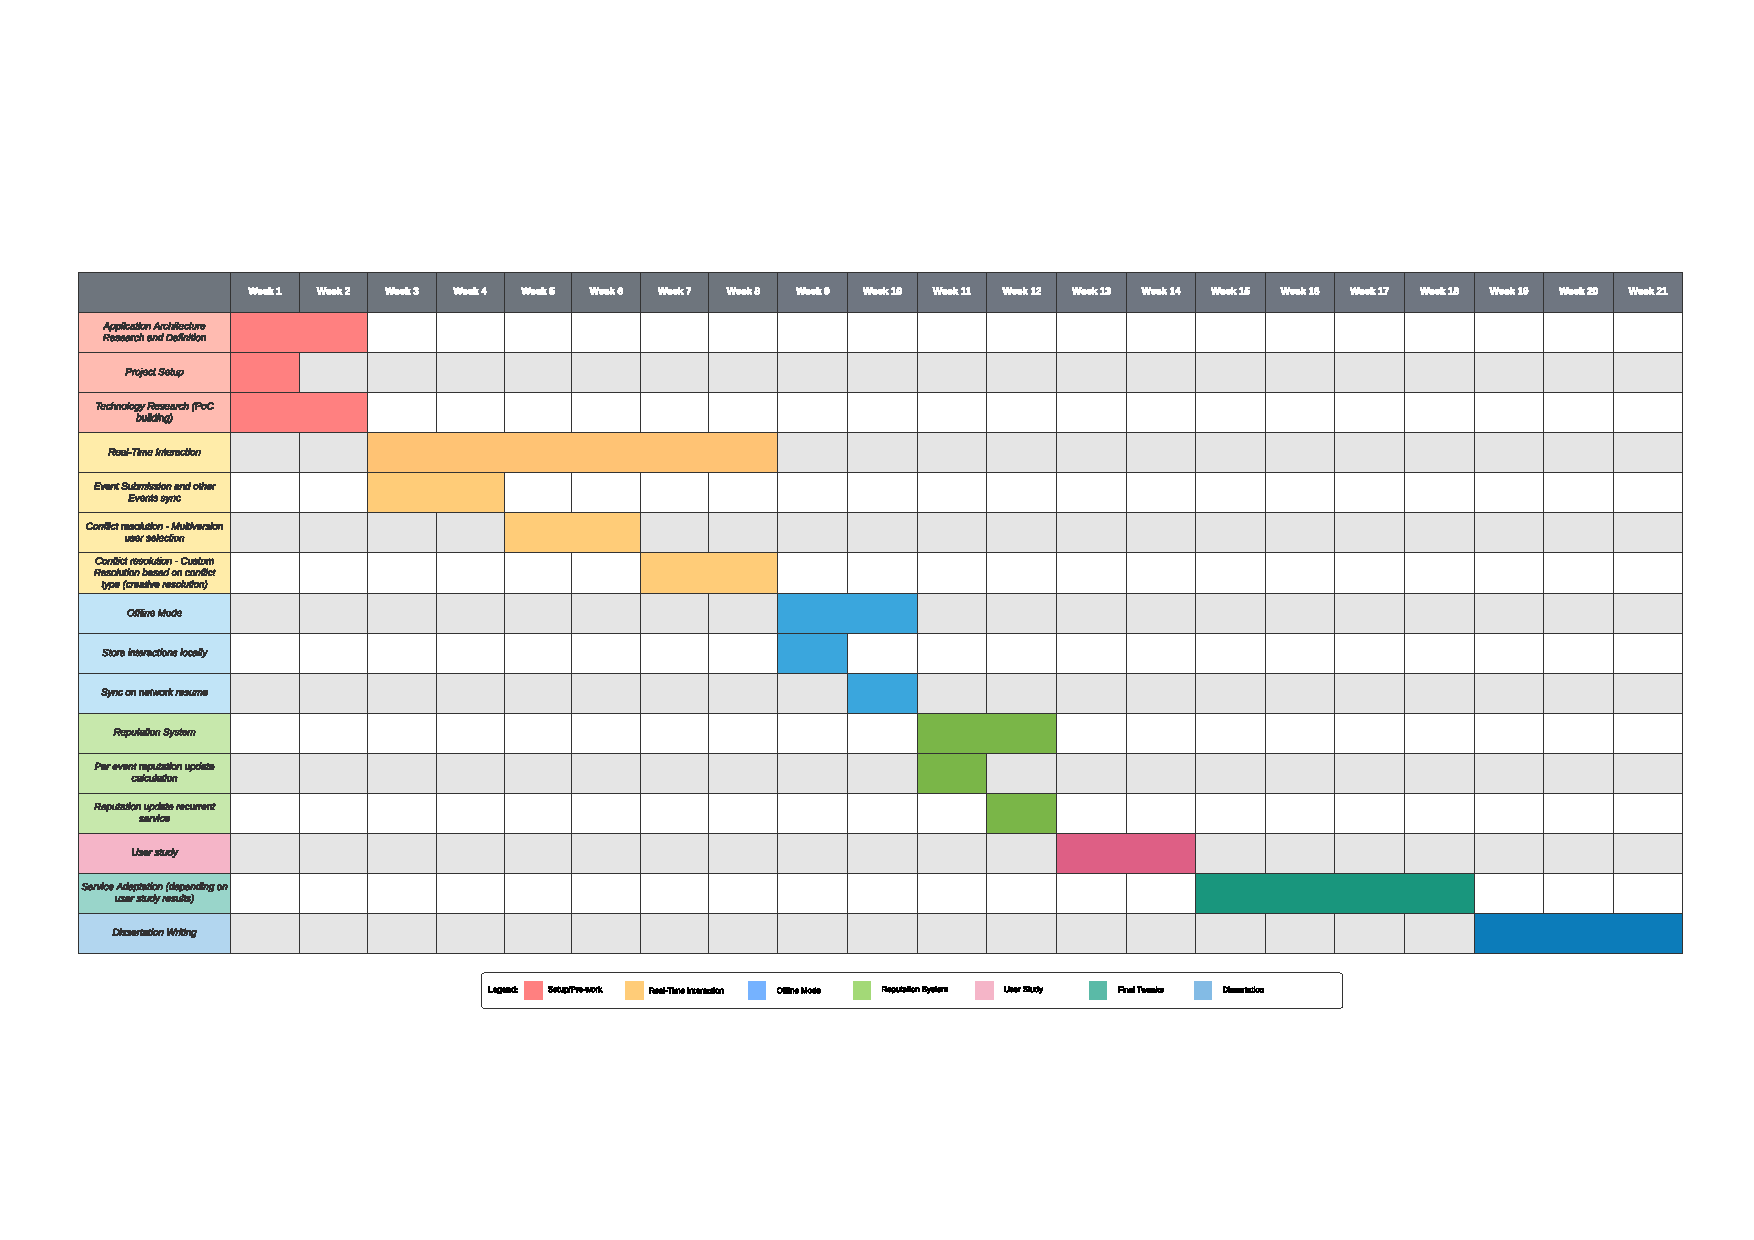
\includegraphics[height=1.0\textheight]{gantt_diss.pdf}
    \caption{Plan Gantt chart}
    \label{fig:gantt-plan}
\end{figure}
\end{landscape}
